\subsection{Gaussian Noise with Salt and Pepper}

By analyzing image 2 in an uniform area it can be seen that the image has both salt and pepper noise, illustrated in figure \ref{fig:hist2_uniform}.

\begin{figure}[H]
\centering
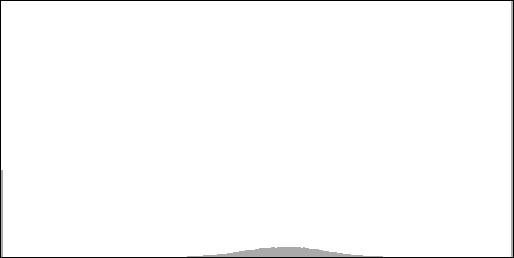
\includegraphics[width = \histogramWidth]{graphics/hist2_uniform.png}
\caption{Histogram of the original ``Image2.png'' showing salt and pepper noise in a uniform area.}
\label{fig:hist2_uniform}
\end{figure}

As in section \ref{image_1} this is removed with a shifted median filter.
The amount of white in the image is 30\% and the amount of black is 10\%.
The quantile was thus chosen to be 40\%.
It was found that a 5x5 filter removed the extreme values but was not efficient at removing the rest of the noise.
A harmonic mean filter is used to remove the remaining salt noise.
In figure \ref{fig:hist2_median_harmonic} can it be seen that the removal of salt and pepper noise was successful.
It can be seen that the two filters removed the white noise.
The black parts is not pepper noise but rather black added from the edge, where the filter takes pixels from outside the image.

\begin{figure}[H]
\centering
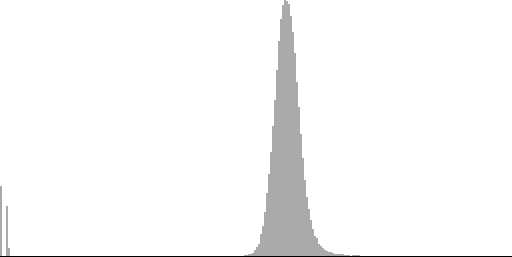
\includegraphics[width = \histogramWidth]{graphics/hist2_after_median.png}
\caption{Histogram of the uniform area after median filter.}
\label{fig:hist2_median_harmonic}
\end{figure}

The variance was found in the uniform area to be $37.3$.
Gaussian noise remains and this was removed with a homomorphic bilateral filter.
A bilateral filter can simplify an image by removing Gaussian noise.
If the image suffers from Gaussian noise, it can be assumed different colors within a variance is supposed to be the same color.
A second parameter for the openCV is the sigma space / intensity space. 
This is kept low to avoid all colors from coming together. 
A value of 3 has been chosen.
In figure \ref{fig:hist2_bilateral} can it be seen that the variance has decreased to $18.2$ so the filter is deemed appropriate.
Because the Gaussian noise is multiplicative, the bilateral filter is applied as a homomorphic filter.

\begin{figure}[H]
\centering
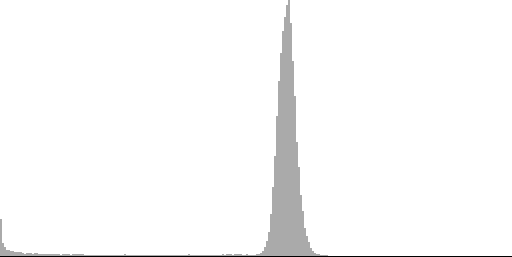
\includegraphics[width = \histogramWidth]{graphics/hist2_after_bilatteral.png}
\caption{Histogram of the uniform area after bilateral filter.}
\label{fig:hist2_bilateral}
\end{figure}

To see the effect of on the complex area, the same filters have been applied to that region.
First the median filter is applied, leading to the image shown in figure \ref{fig:complex2_median}.
Then the harmonic filter is applied, shown in figure \ref{fig:complex2_harmonic}.
Then the bilateral filter is applied, shown in figure \ref{fig:complex2_bilatteral}.

\begin{figure}[H]
\centering
  \begin{subfigure}{\linewidth}
  \centering
    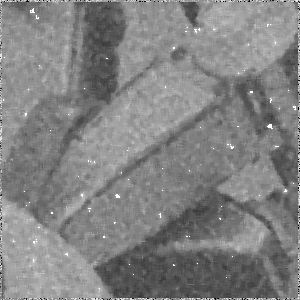
\includegraphics[width = \cutOutWidth]{graphics/complex2_median.png}
    \caption{After median filter.}
    \label{fig:complex2_median}
  \end{subfigure}
  
  \begin{subfigure}{\cutOutWidth}
  \centering
    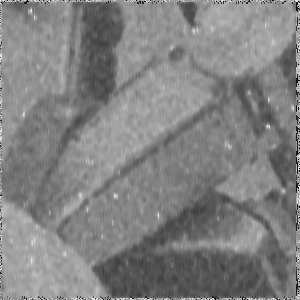
\includegraphics[width = \linewidth]{graphics/complex2_harmonic.png}
    \caption{After harmonic filter.}
    \label{fig:complex2_harmonic}
  \end{subfigure}
  \begin{subfigure}{\cutOutWidth}
  \centering
    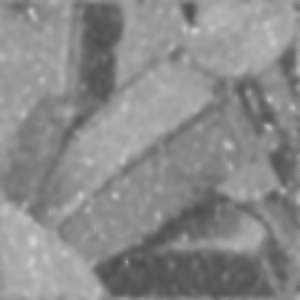
\includegraphics[width = \linewidth]{graphics/complex2_bilatteral.png}
    \caption{After bilatteral filter.}
    \label{fig:complex2_bilatteral}
  \end{subfigure}
  \caption{The complex area in the different stages.}
\end{figure}

It can be seen that the image lacks contrast.
The lack of contrast can be added with a histogram equalization scheme.
The histogram equalization stretches the color values to the extremes and thus the image quality does not improve.
So before the histogram equalization, a alpha trimmed mean with the kernel size of 7x7 and mean width of 3 is applied to remove further extreme values.
In figure \ref{fig:complex2_histeq_smoothed} can the image be seen after alpha trimmed smoothed and then histogram equalization.

\begin{figure}[H]
\centering
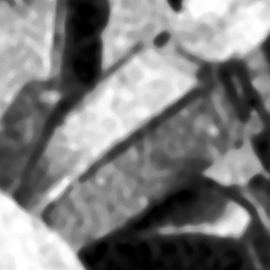
\includegraphics[width = \cutOutWidth]{graphics/complex2_histeq_smoothed.png}
\caption{Histogram equalization of the smoothed compex area.}
\label{fig:complex2_histeq_smoothed}
\end{figure}

This still adds a lot of noise to the image. 
The contrast improves but since the contrast is too small to begin with, giving high contrast in areas where there should be none.

The resulting sequence is thus:
\begin{itemize}
 \item Shifted median filter, kernel size 5x5, quantile of 40\%.
 \item Harmonic mean filter, kernel size 5x5.
 \item Homomorphic bilateral filter, kernel size 11x11, variance of $37.3$, depth of 3.
\end{itemize}
The resulting image restoration of image 2 can be seen in figure \ref{fig:image_2_restored}.

\begin{figure}[H]
\centering
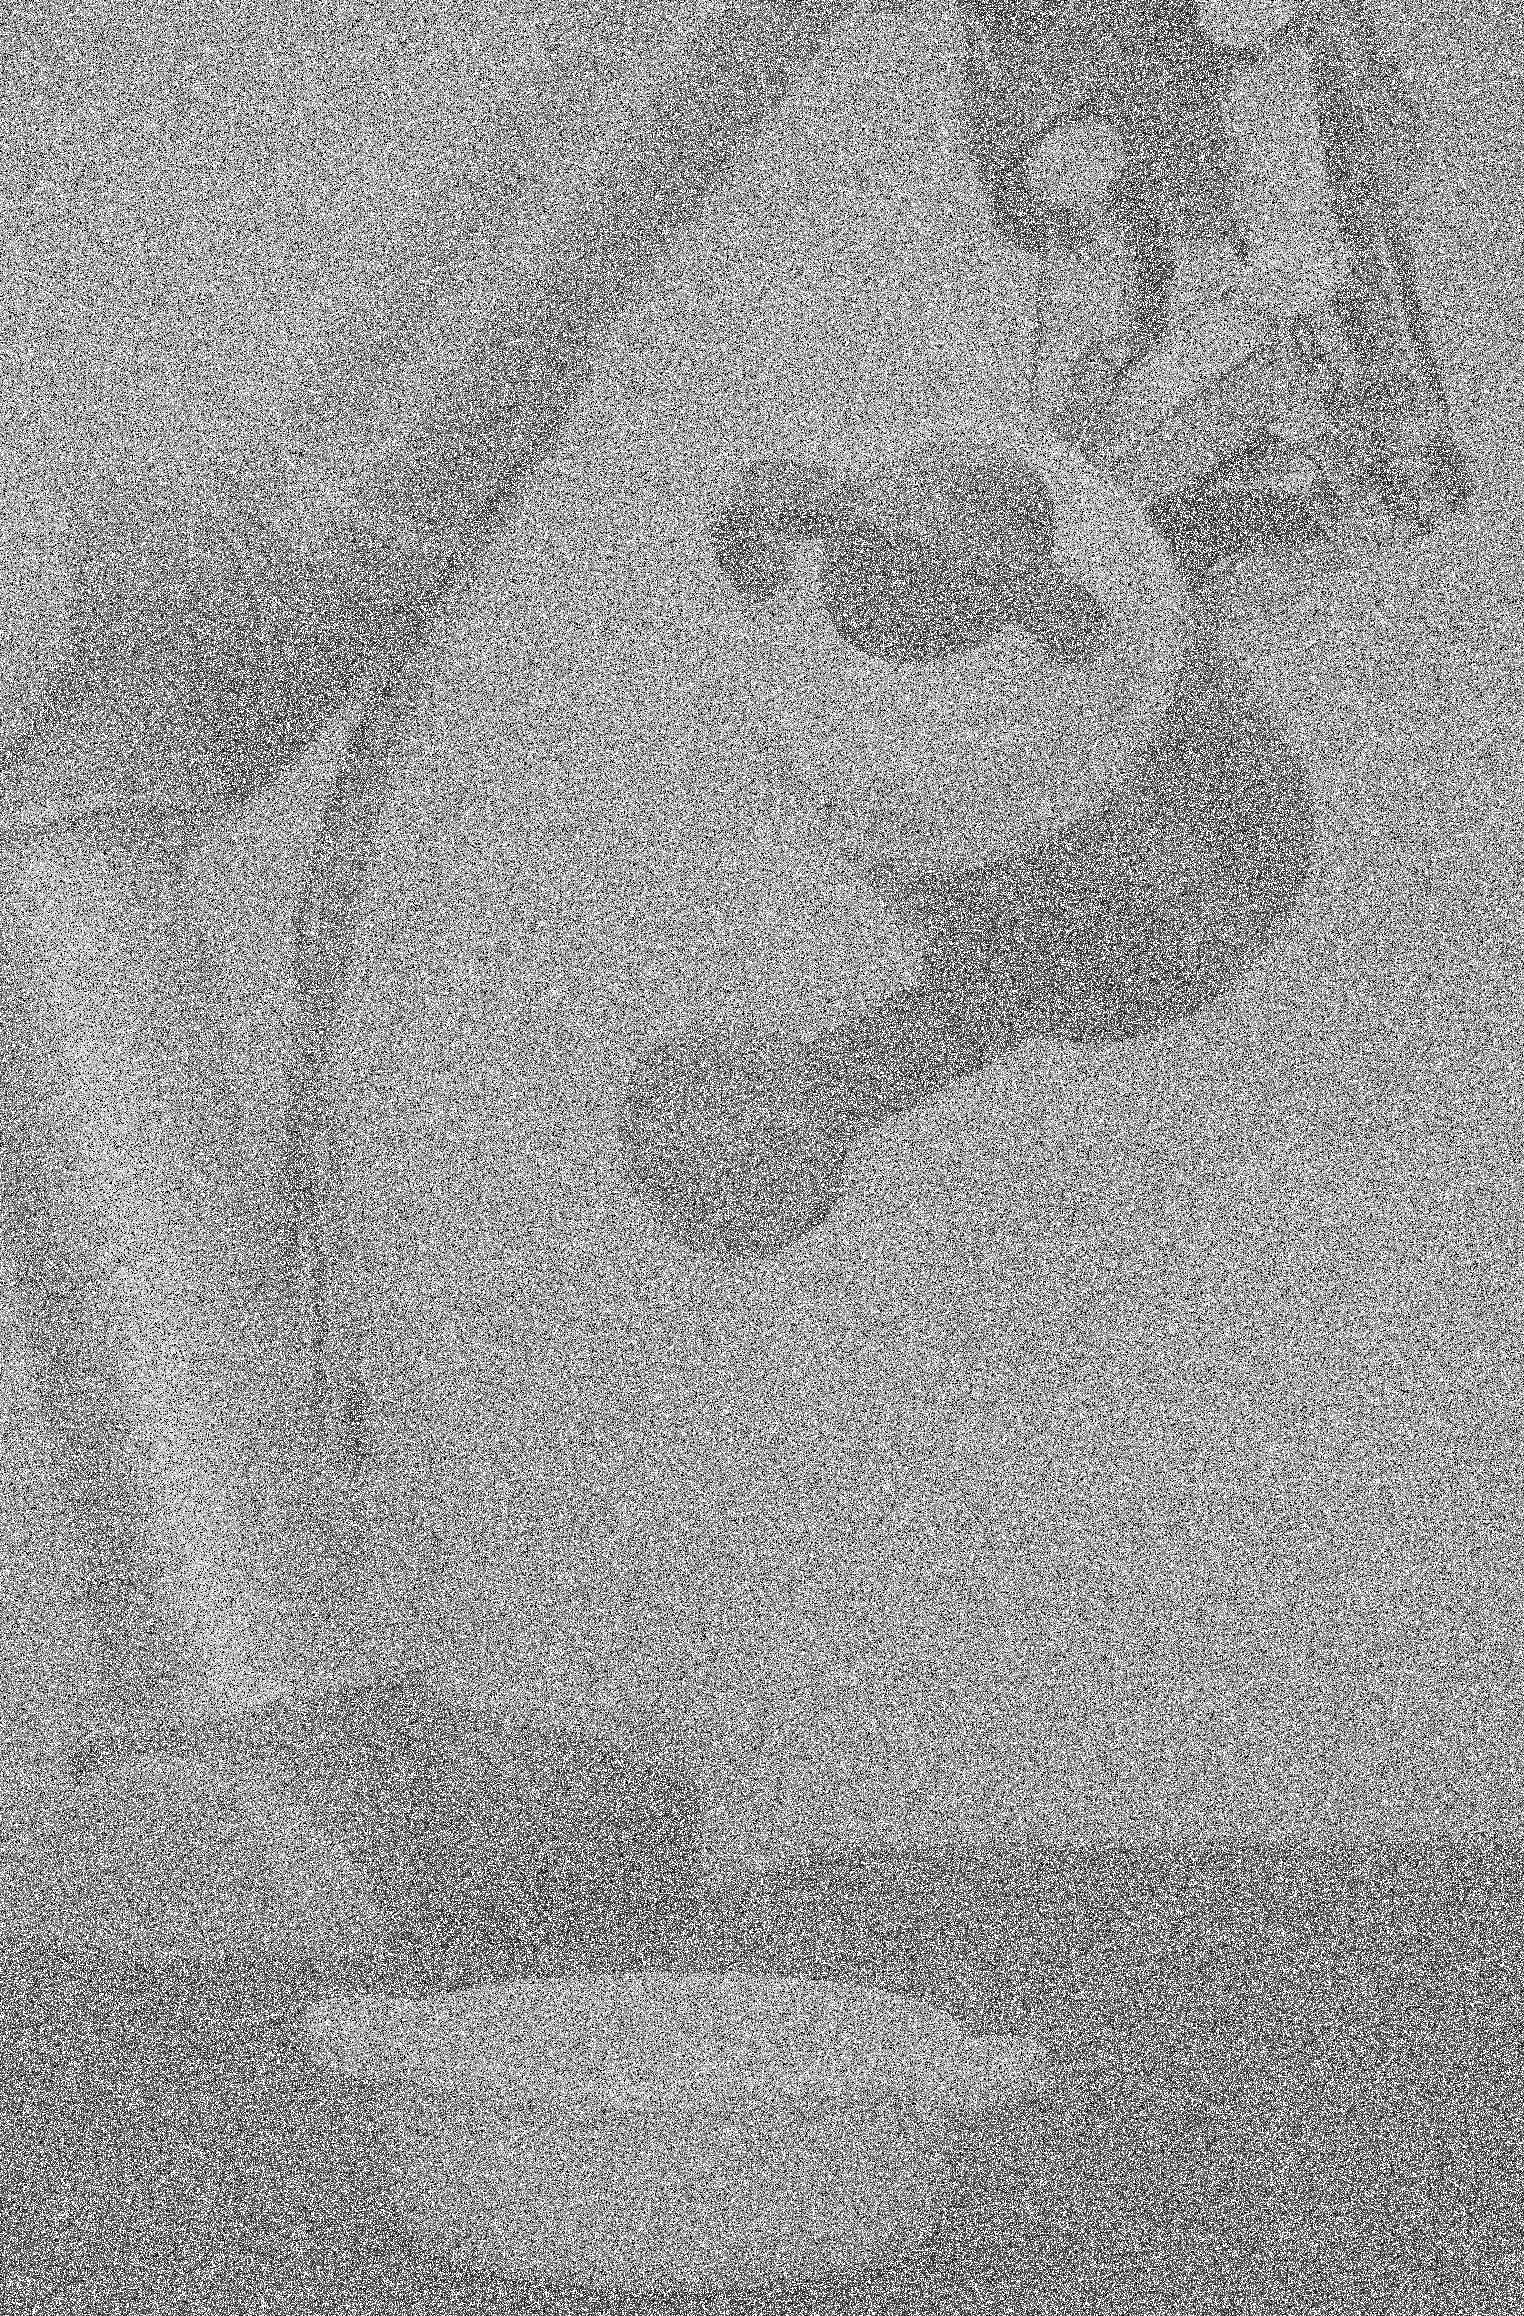
\includegraphics[width = \fullImageWidth]{../code/images/image_result_2.png}
\caption{The restored image 2.}
\label{fig:image_2_restored}
\end{figure}
